\documentclass{beamer}
\usepackage[utf8]{inputenc}
\usepackage{amsmath, pdfpages, pdflscape, lscape, color, listings, hyperref, amssymb, graphicx,textcomp,varioref, afterpage, subcaption, float, bm, tikz, multicol} 


\newcommand{\Fig}[1]{Figure \ref{#1}}
\newcommand{\fig}[1]{figure \ref{#1}}
\newcommand{\tab}[1]{table \ref{#1}}
\newcommand{\eq}[1]{equation \ref{#1}}
\newcommand{\Eq}[1]{Equation \ref{#1}}
\newcommand{\alg}[1]{algorithm \ref{#1}}
\newcommand{\Alg}[1]{Algorithm \ref{#1}}
\newcommand{\chp}[1]{chapter  \ref{#1}}
\newcommand{\Chp}[1]{Chapter  \ref{#1}}
\newcommand{\e}[1]{\cdot 10^{#1}}
\newcommand{\h}{\hbar}
\newcommand{\der}[2]{\frac{\partial #1}{\partial #2}}
\newcommand{\dder}[2]{\frac{\partial^2 #1}{\partial #2^2}}
\newcommand{\p}{\boldsymbol{P}}
\newcommand{\q}{\boldsymbol{q}}
\newcommand{\norm}[1]{\left\lVert#1\right\rVert}
\newcommand{\coef}[2]{\frac{\langle #1,#2\rangle_Q}{\norm{#2}^}}


\newenvironment{test}[1]
{
 \usebackgroundtemplate{}
 \color{gray!30!black}
   \begin{tikzpicture}[remember picture, overlay]
     \node[anchor = center, opacity=.25] (image) at (current page.center) {
\includegraphics[scale=0.25]{chaospy_logo.jpg}};
   \end{tikzpicture}
 \begin{frame}[fragile,enviroment=chaospy]
   
}
{
 \end{frame}
}


\newenvironment{chaospy}[1]
{\color{gray!30!black}
     \color{gray!30!black}
     \usebackgroundtemplate{
   \begin{tikzpicture}[remember picture, overlay]
     \node[anchor = center, opacity=.25] (image) at (current page.center) {
\includegraphics[scale=0.25]{chaospy_logo.jpg}};
   \end{tikzpicture}}
     \begin{frame}[fragile,environment=chaospy]
    \frametitle{{#1}}}
{\end{frame}}


\definecolor{keywords}{RGB}{255,0,90}
\definecolor{comments}{RGB}{0,0,113}
\definecolor{red}{RGB}{160,0,0}
\definecolor{green}{RGB}{0,150,0}
 
\usetheme{kalkulo}

\graphicspath{{./figures/}}


\title{Polynomial chaos expansions part 2: Practical Implementation}
\author{Jonathan Feinberg and Simen Tennøe}


\begin{document}



\begin{frame}
  \maketitle
\end{frame}

\begin{frame}
 \frametitle{Repetition: The problem}
  We have a simple differential equation
  \begin{align*}
    \frac{d u(x)}{dx} & =-au(x),\qquad u(0) = I,
  \end{align*}
  where $a$ and $I$ are uncertain.
\end{frame}


\begin{chaospy}{Repetition: The 1D code, with a uncertain and $I=1$}
 \begin{lstlisting}[language=python]
a = cp.Uniform(0,0.1)

def u(x,a):
  ax = np.outer(a,x)
  return np.exp(-ax)

m = 5
x = np.linspace(0, 10, 100)

P = cp.orth_ttr(m, a)
nodes, weights = cp.generate_quadrature(m+1, a,
                                        rule="G")
solves = u(x,nodes[0])
U_hat = cp.fit_quadrature(P, nodes,
                          weights, solves)
\end{lstlisting}
\end{chaospy}


\begin{frame}
 \frametitle{Plot of convergence}
 \begin{figure}
  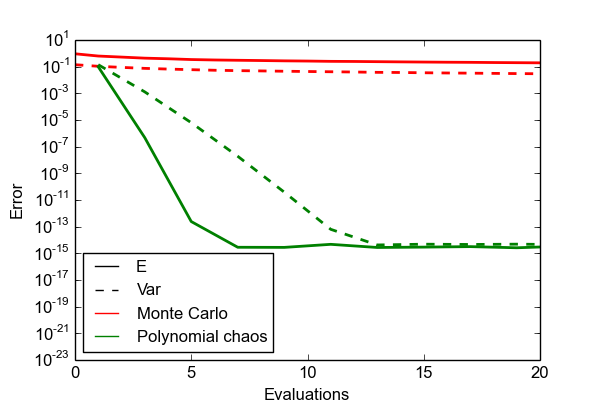
\includegraphics[width=0.8\textwidth]{Convergence_repeat.png}
 \end{figure}

\end{frame}



\begin{frame}
 \frametitle{The pseudo spectral approach: how I stopped worrying and learned to calculate the fourier coefficients}

 \begin{align*}
 c_i(x) &= \frac{\langle P_i,u(x,q)\rangle}{\norm{P_i}^2}\\
 &=\frac{1}{\norm{P_i}^2} \int P_i(q)u(x,q)f(q)dq \approx\\
 \pause
  \hat{c}_i(x) &= \sum P_i(q_k)f(q_k)\omega_k  
\end{align*}
$q_k$ - quadrature nodes
$\omega_k$ - quadrature weights
 \end{frame}
 
\begin{chaospy}{Repetition: 2D code}
   \begin{lstlisting}[language=python]
def u(x,a, I):
  return I*np.exp(-a*x)
 
a = cp.Uniform(0, 0.1)
I = cp.Uniform(8, 10)
dist = cp.J(a,I)
x = np.linspace(0, 10, 100); k = 4; m = 5

P = cp.orth_ttr(m, dist)
nodes, weights = cp.generate_quadrature(k, dist, 
                                       rule="E")
i1,i2 = np.mgrid[:len(weights), :Nt]
solves = u(x[i2],nodes[0][i1],nodes[1][i1])
U_hat = cp.fit_quadrature(P, nodes, weights,
                          solves)
\end{lstlisting}
\end{chaospy}


\begin{frame}
 \frametitle{Plot of the nodes for a 2D problem}
 \begin{figure}
  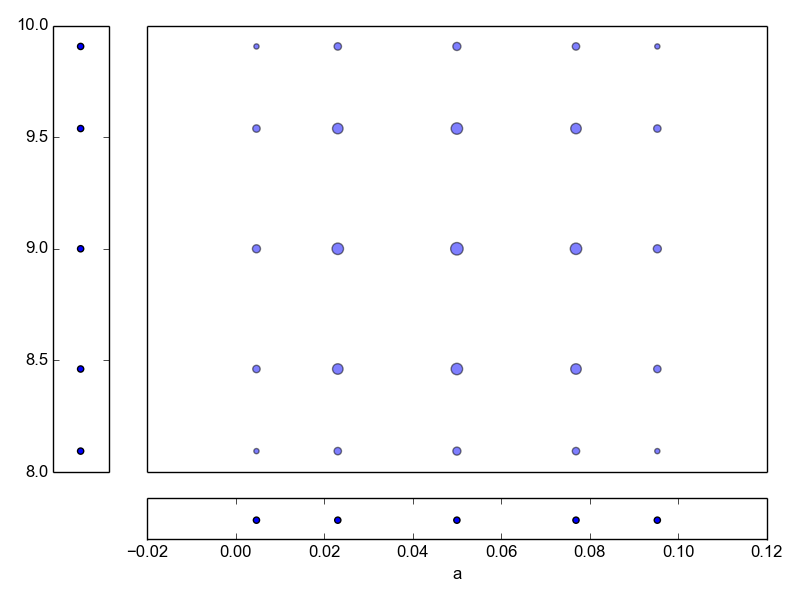
\includegraphics[width=0.85\textwidth]{nodes.png}
 \end{figure}
\end{frame}


\begin{frame}
 \frametitle{The number of nodes goes as, $k = (N+1)^D$}
 \begin{figure}
  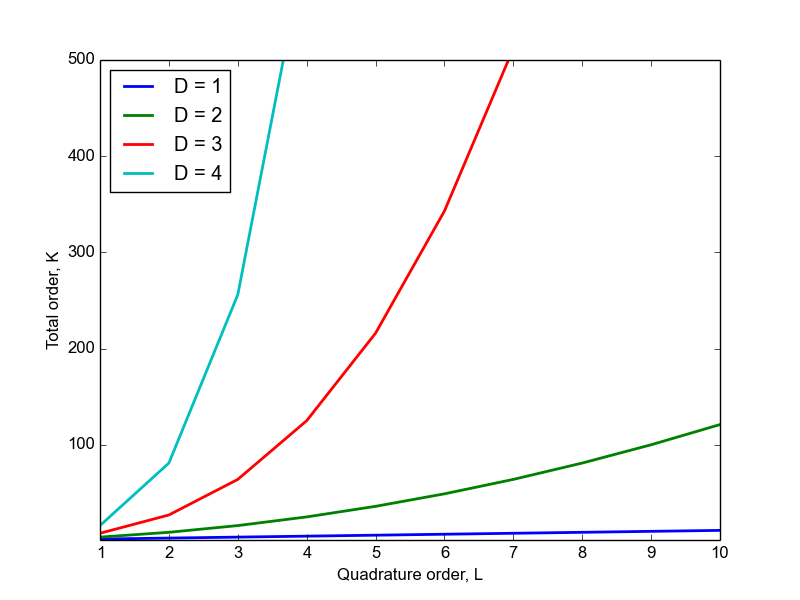
\includegraphics[width=0.85\textwidth]{dimensionality_nodes.png}
 \end{figure}
\end{frame}

\begin{frame}[fragile]
 \frametitle{Plot of the nodes for a 2D problem using a sparse grid}
 \begin{lstlisting}[language=python]
  nodes, weights = 
   cp.generate_quadrature(k, dist, 
   rule="E", sparse=True)
 \end{lstlisting}

 \pause
 \begin{figure}
  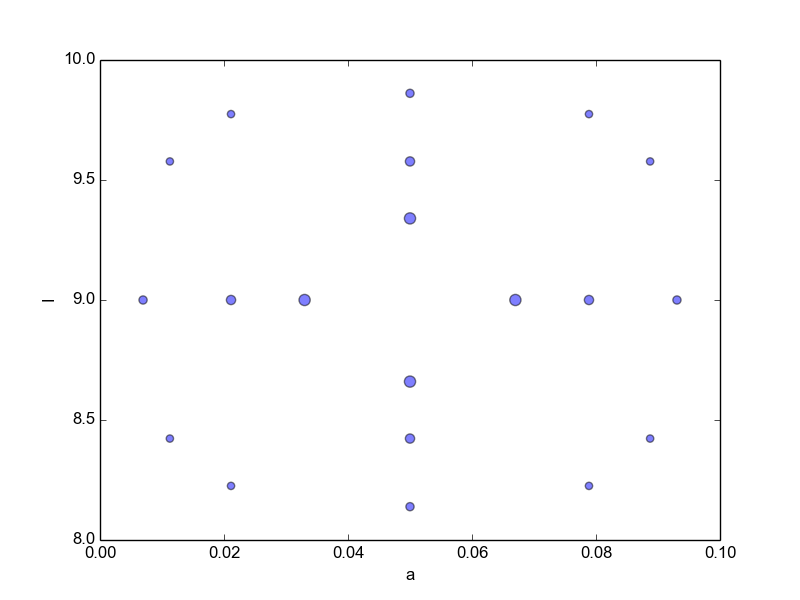
\includegraphics[width=0.6\textwidth]{nodes_sparse.png}
 \end{figure}
\end{frame}
 
 
 \begin{frame}
  \frametitle{Nested sparse grids}
 Clenshaw-Curtis: cp.generate\_quadrature(k, dist, rule="C",growth=False)
  \begin{table}
  \begin{tabular}{lcccccccc}
    1& &&& $\bullet$& &&&  \\\hline
   2 &&&$\bullet$& &$\bullet$&&& \\\hline
   3 &&$\bullet$&&$\bullet$ &&$\bullet$&& \\
   \end{tabular}
  \end{table}
  
  
  Nested Clenshaw-Curtis: cp.generate\_quadrature(k, dist, rule="C",growth=True)
  \begin{table}
  \begin{tabular}{lcccccccc}
    1& &&& $\bullet$& &&&  \\\hline
   2 &&$\bullet$&& $\bullet$&&$\bullet$ && \\\hline
   3 &$\bullet$&$\bullet$&$\bullet$& $\bullet$&$\bullet$&$\bullet$ &$\bullet$& \\
   \end{tabular}
  \end{table}
 
  \end{frame}



 
 \begin{frame}
 \frametitle{Clenshaw-Curtis quadrature vs Gaussian quadrature}
 \begin{figure}        
 \begin{subfigure}[b]{0.5\textwidth}
                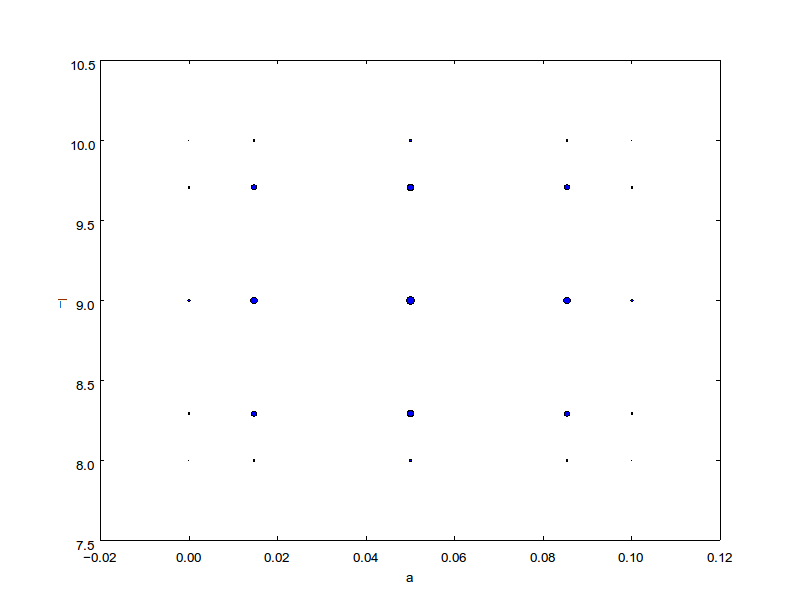
\includegraphics[width=\textwidth]{nodes_C.png}
                \caption{Clenshaw-Curtis quadrature}
        \end{subfigure}%        
 \begin{subfigure}[b]{0.5\textwidth}
                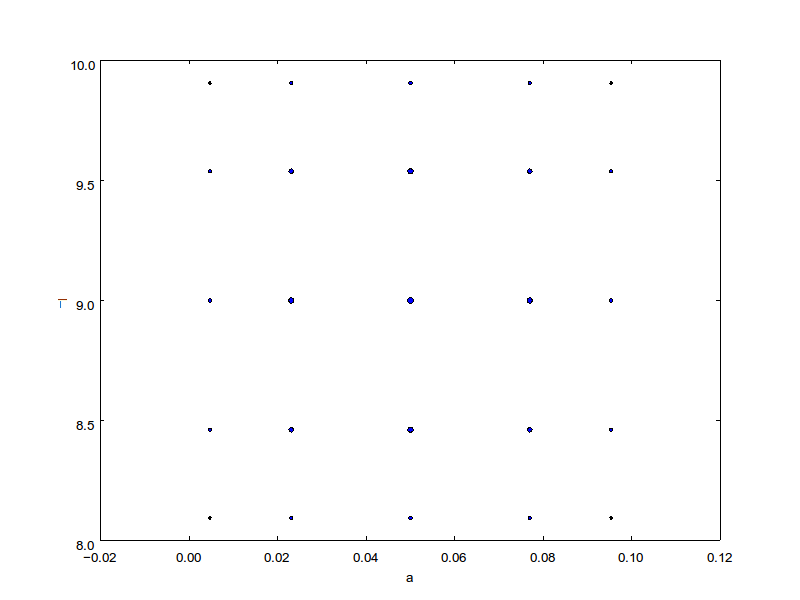
\includegraphics[width=\textwidth]{nodes_G.png}
                \caption{Gaussian quadrature}
        \end{subfigure}
        \end{figure}
\end{frame}
 
 
 \begin{frame}
  \frametitle{Number of nodes needed}
  \begin{itemize}
   \item $L$ is the number of nodes along one axis
  \end{itemize}

 \begin{figure}
  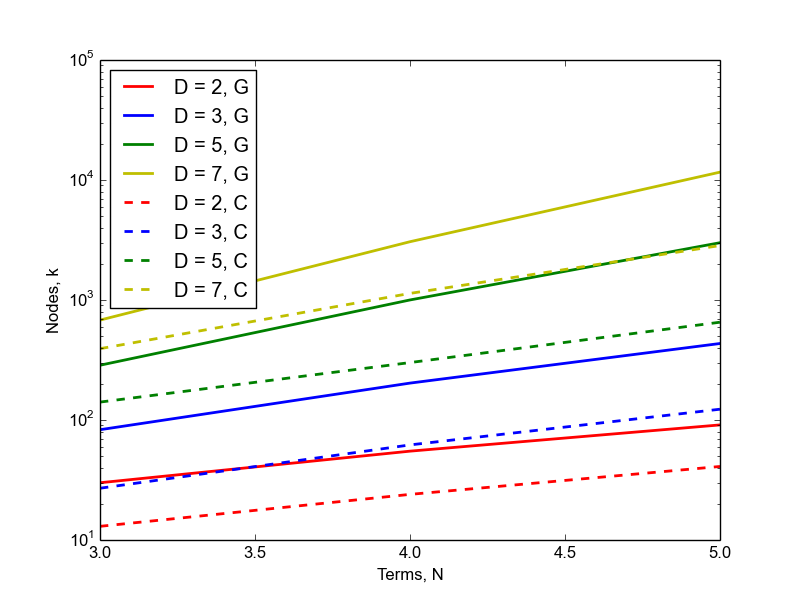
\includegraphics[width=0.85\textwidth]{dimensionality_nodes_sparse.png}
 \end{figure}
 \end{frame}

  
  \begin{frame}
   \frametitle{Mapping between order, M and number of nodes , L}
   For nested Clenshaw-Curtis
   \begin{figure}
    \includegraphics<1>[width=0.85\textwidth]{LvsM1.png}
    \includegraphics<2>[width=0.85\textwidth]{LvsM.png}
   \end{figure}

   
  %\begin{tabular}{lccccccccccc}
  % Order, M & 0 & 1 & 2 & 3 & 4 & 5 & 6 & 7 & 8 \\\\
  % Quad  & 1 & 4 & 9 & 16 & 25 & 36 & 49 & 64 & 81 \\\\
  % Poly  & 1 & 3 & 6 & 10 & 15 & 21 & 28 & 37 & 37
  %\end{tabular}

  \end{frame}

  
  
 \begin{frame}
  \frametitle{Definition of Gaussian quadrature}
  \begin{align*}
   \int W(q)u(x,q)dq &\approx \sum_k \omega_k u(x,q_k)\\
   \intertext{for a fitting $W(q)$}
   \pause
   \int f(q)u(x,q)dq &\approx \sum_k \omega_k u(x,q_k)\\
     \end{align*}
 \end{frame}

 
  \begin{frame}
 \frametitle{Different distributions}
 \begin{figure}        
 \begin{subfigure}[b]{0.37\textwidth}
                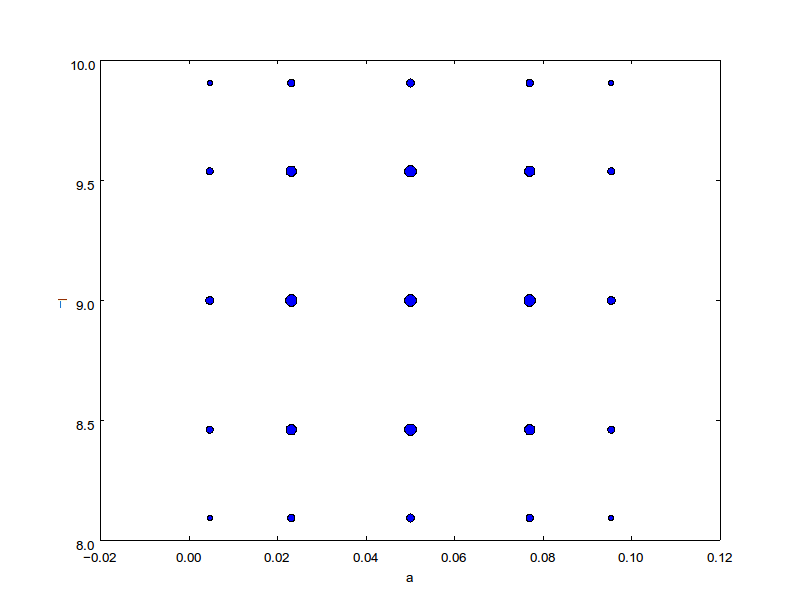
\includegraphics[width=\textwidth]{nodes_uniform.png}
                \caption{Uniform}
        \end{subfigure}%        
 \begin{subfigure}[b]{0.37\textwidth}
                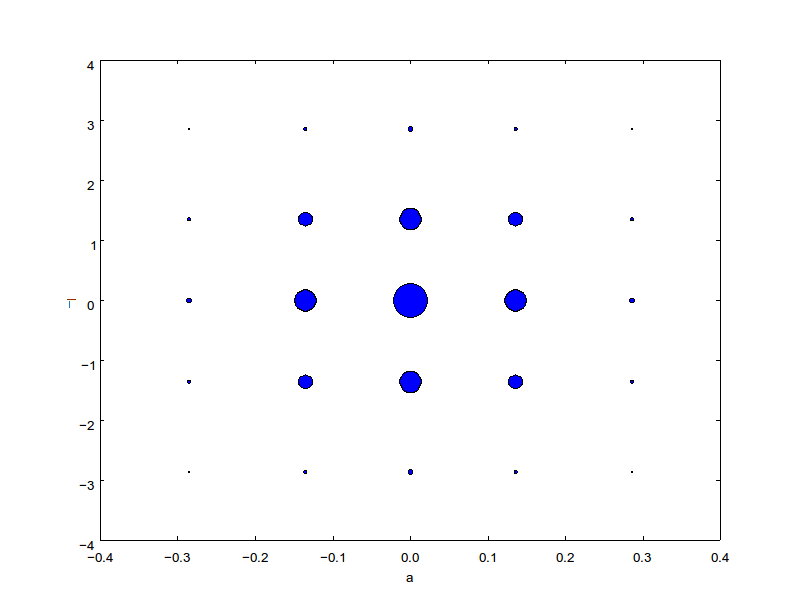
\includegraphics[width=\textwidth]{nodes_normal.png}
                \caption{Normal}
        \end{subfigure}
 \begin{subfigure}[b]{0.37\textwidth}
                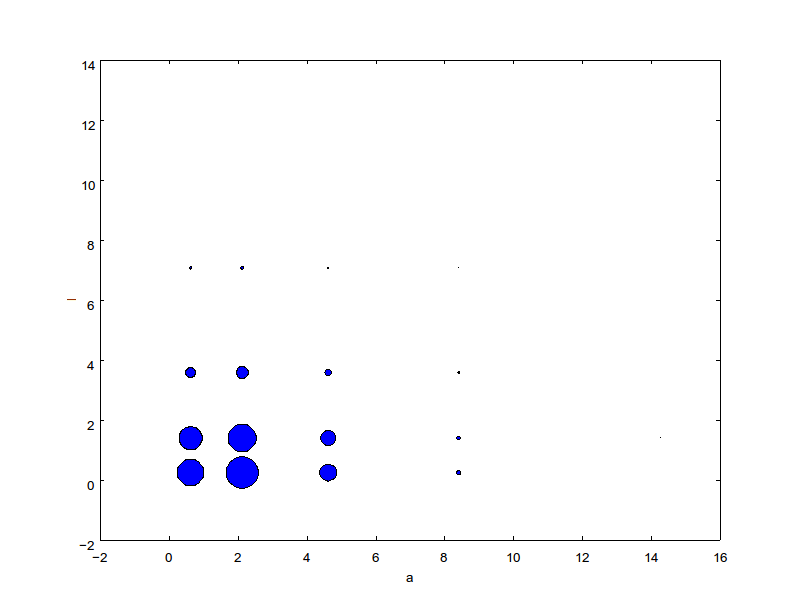
\includegraphics[width=\textwidth]{nodes_gamma.png}
                \caption{Gamma}
        \end{subfigure}%        
 \begin{subfigure}[b]{0.37\textwidth}
                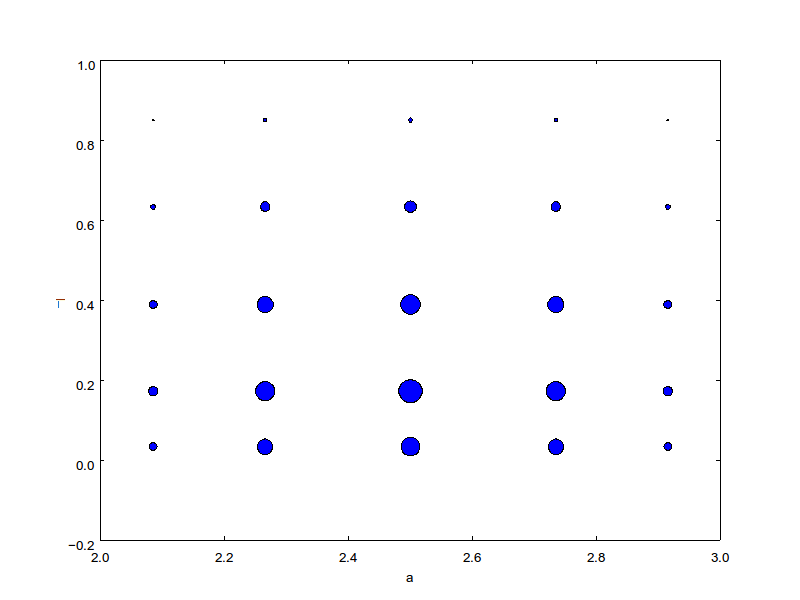
\includegraphics[width=\textwidth]{nodes_beta.png}
                \caption{Beta}
        \end{subfigure}
        \end{figure}
               
\end{frame}
 
 
 \begin{frame}
  \frametitle{Convergence for Gaussian quadrature vs Legendre}
  \begin{figure}
   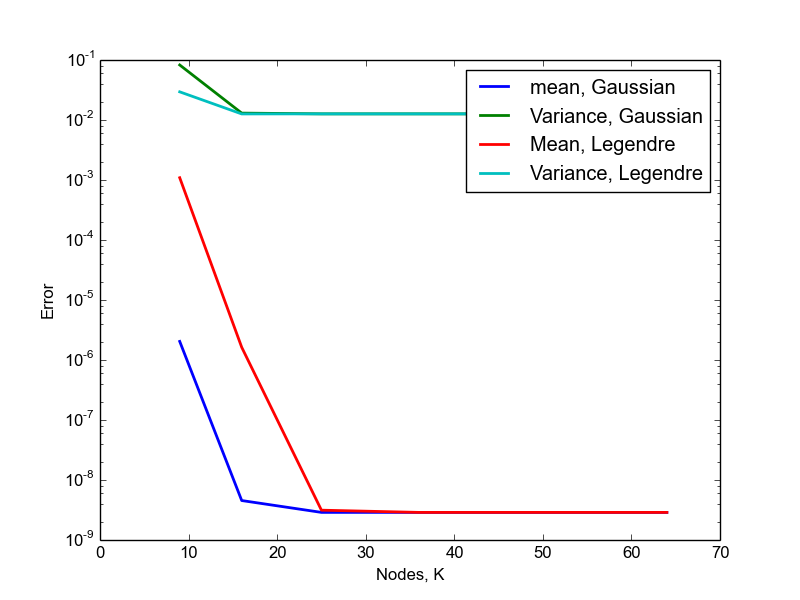
\includegraphics[width=0.85\textwidth]{convergence_GvsL.png}
  \end{figure}

 \end{frame}

 \if f
 \begin{frame}
  \frametitle{Point collocation}
  
  \begin{align*}
   \overrightarrow{C} = \left[
  \begin{matrix}
  C_0  \\
  \vdots \\
  C_N 
 \end{matrix}\right]
 
 && \overrightarrow{P} = \left[
  \begin{matrix}
  P_0(q_0) & \dots & P_N(q_0)  \\
  \vdots & & \vdots \\
  P_0(q_k) & \dots& P_N(q_k) 
 \end{matrix}\right]
  \end{align*}

 
   \[\overrightarrow{U} = \left[
  \begin{matrix}
  u(x,q_0)  \\
  \vdots \\
  u(x,q_k) 
 \end{matrix}\right]\]
 \end{frame}

 \fi
 
 
 
 
 
%\begin{chaospy}{Testing the very basics}
% \begin{alert}{Exercise:}
%The voltage, V, over a capacitator in a RC circuit is given by:
% \[V_0e^{-\frac{t}{\tau}}\]
% where $V_0 = 4$ is the initial condition and $\tau$ the time constant. Our measurments are not precise and $\tau$ is therefore given by a normal distribution around 2
% \end{alert}
%\end{chaospy}





\end{document}
